\documentclass[]{../template/Report}%方括号内写yuxi即生成预习报告\documentclass[yuxi]{../template/Report}
\settemplatedir{../template/}%设置模板路径

\exname{示波器的应用} %实验名称
\extable{9} %实验桌号
\instructor{王鲲} %指导教师
\class{微电子2401} %班级
\name{黄千格} %姓名
\stuid{3240100650} %学号

\nyear{2025} %年
\nmonth{12} %月
\nday{29} %日
\nweekday{一} %星期几，e.g. \nweekday{三}
\daypart{上午}%上午/下午

\redate{} %如有实验补做，补做日期
\resitu{} %情况说明：

\begin{document}
\maketitle%输出封面

\section{预习报告（10分）}
上课前到学在浙大上完成，注意测试仅1次机会。期末时测试分数会与报告其他部分的分数进行加和处理。

\section{原始数据（20分）}
（将有老师签名的“自备数据记录草稿纸”的扫描或手机拍摄图粘贴在下方，完整保留姓名，学号，教师签字和日期。）

\section{结果与分析（60分）}
\subsection{数据处理与结果（30分）}
（列出数据表格、选择适合的数据处理方法、写出测量或计算结果。）
\subsubsection{用比较法验证$f_y = n \cdot f_x$}
示波器波形如下：
\begin{figure}[H]
    \centering

    % --- 第一行 ---
    \begin{subfigure}[b]{0.32\textwidth}
        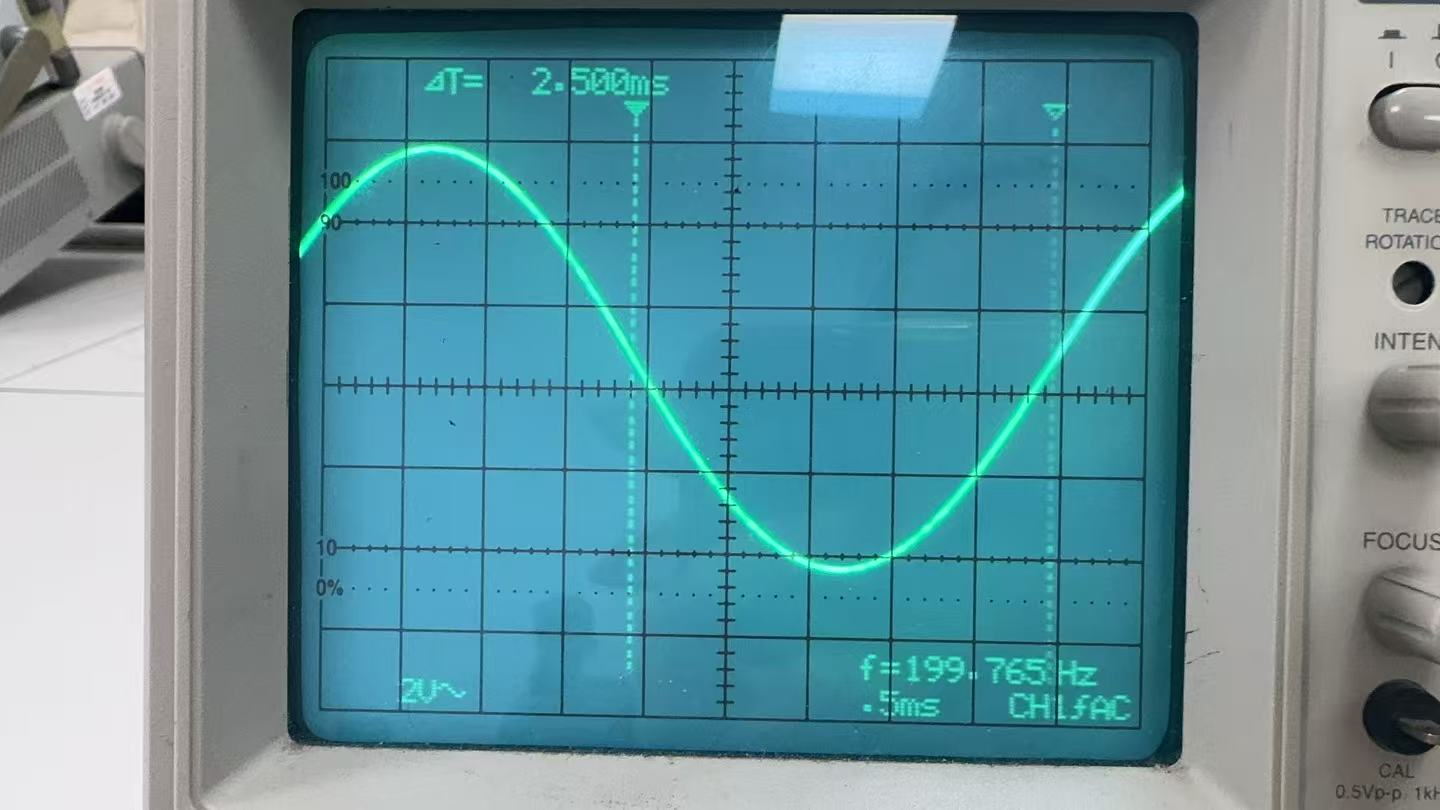
\includegraphics[width=\textwidth]{figures/1-1.jpg}
        \caption{1个完整波形}
        \label{pic:1:1}
    \end{subfigure}
    \hfill % 在子图之间添加水平间距
    \begin{subfigure}[b]{0.32\textwidth}
        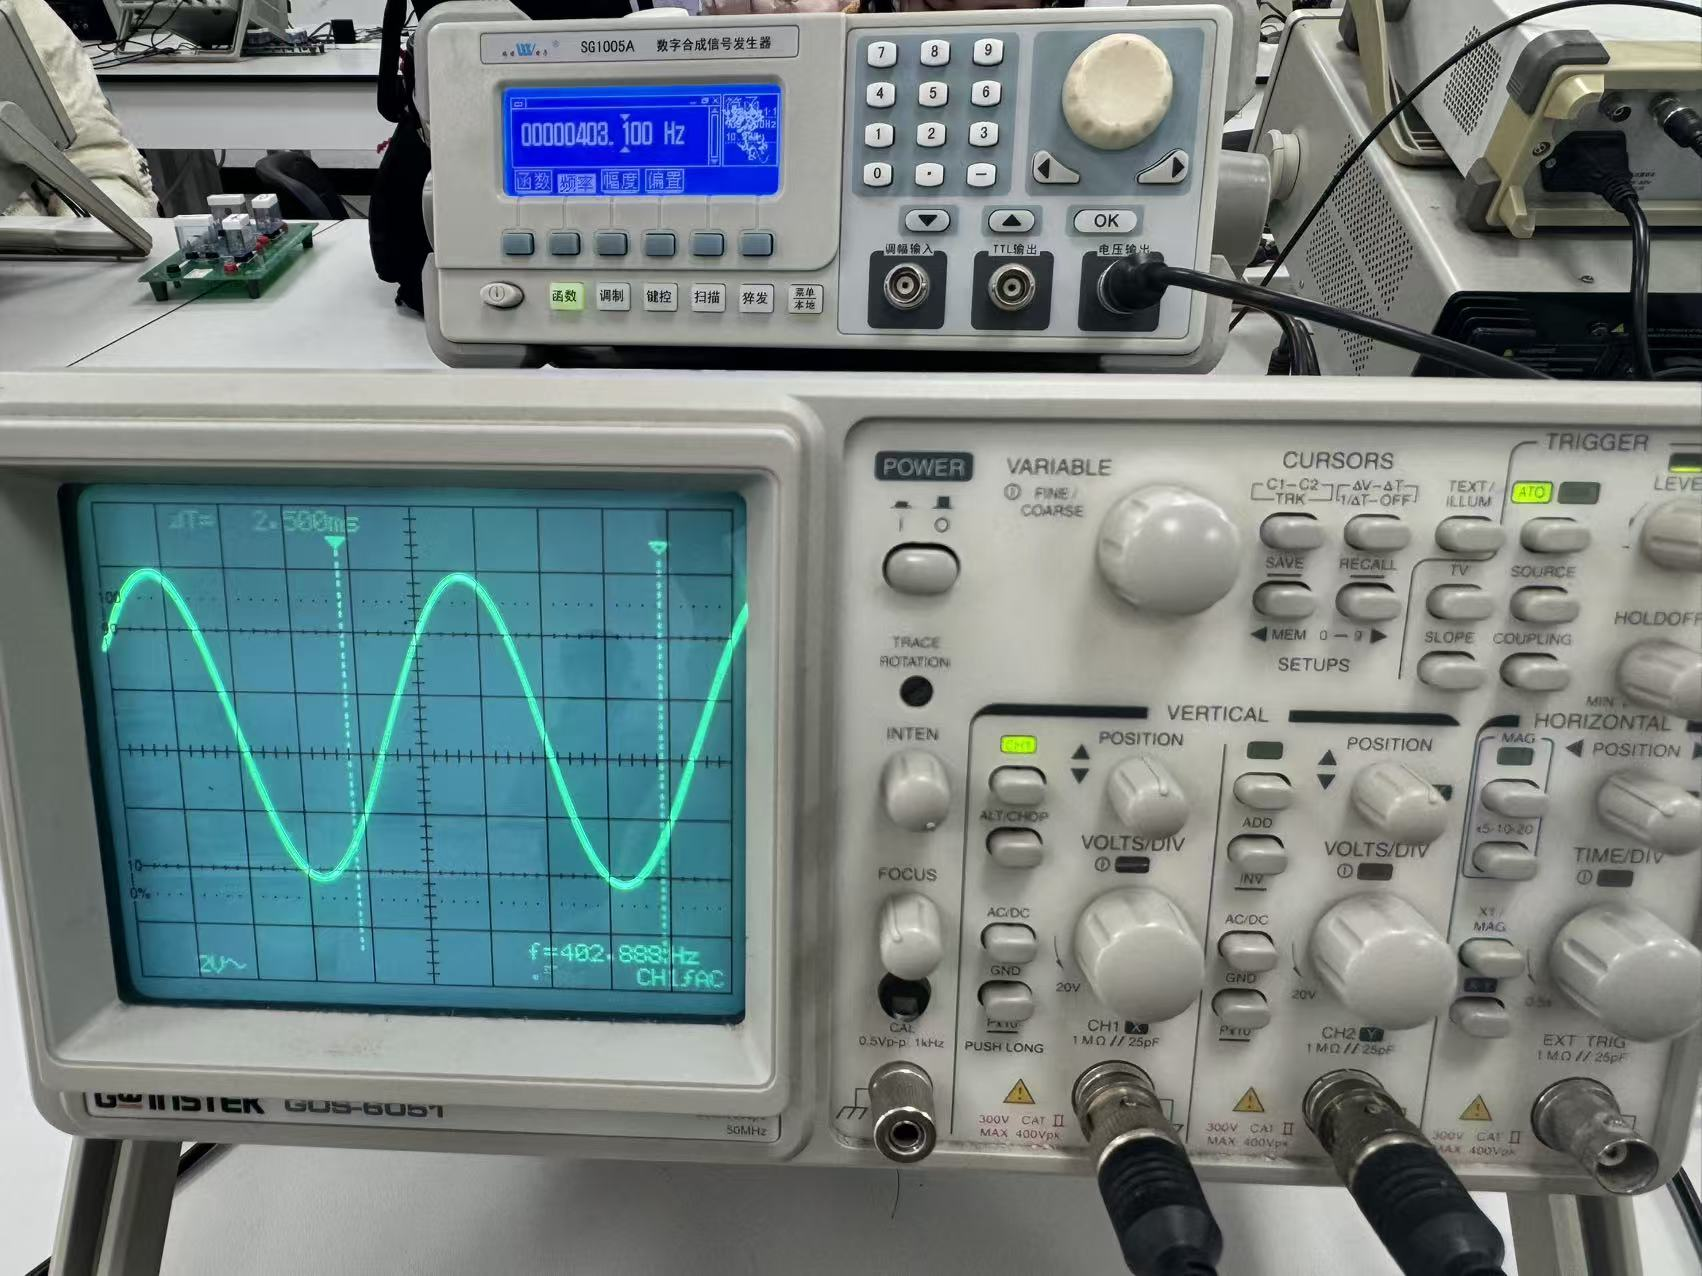
\includegraphics[width=\textwidth]{figures/1-2.jpg}
        \caption{2个完整波形}
        \label{pic:1:2}
    \end{subfigure}
    \hfill % 在子图之间添加水平间距
    \begin{subfigure}[b]{0.32\textwidth}
        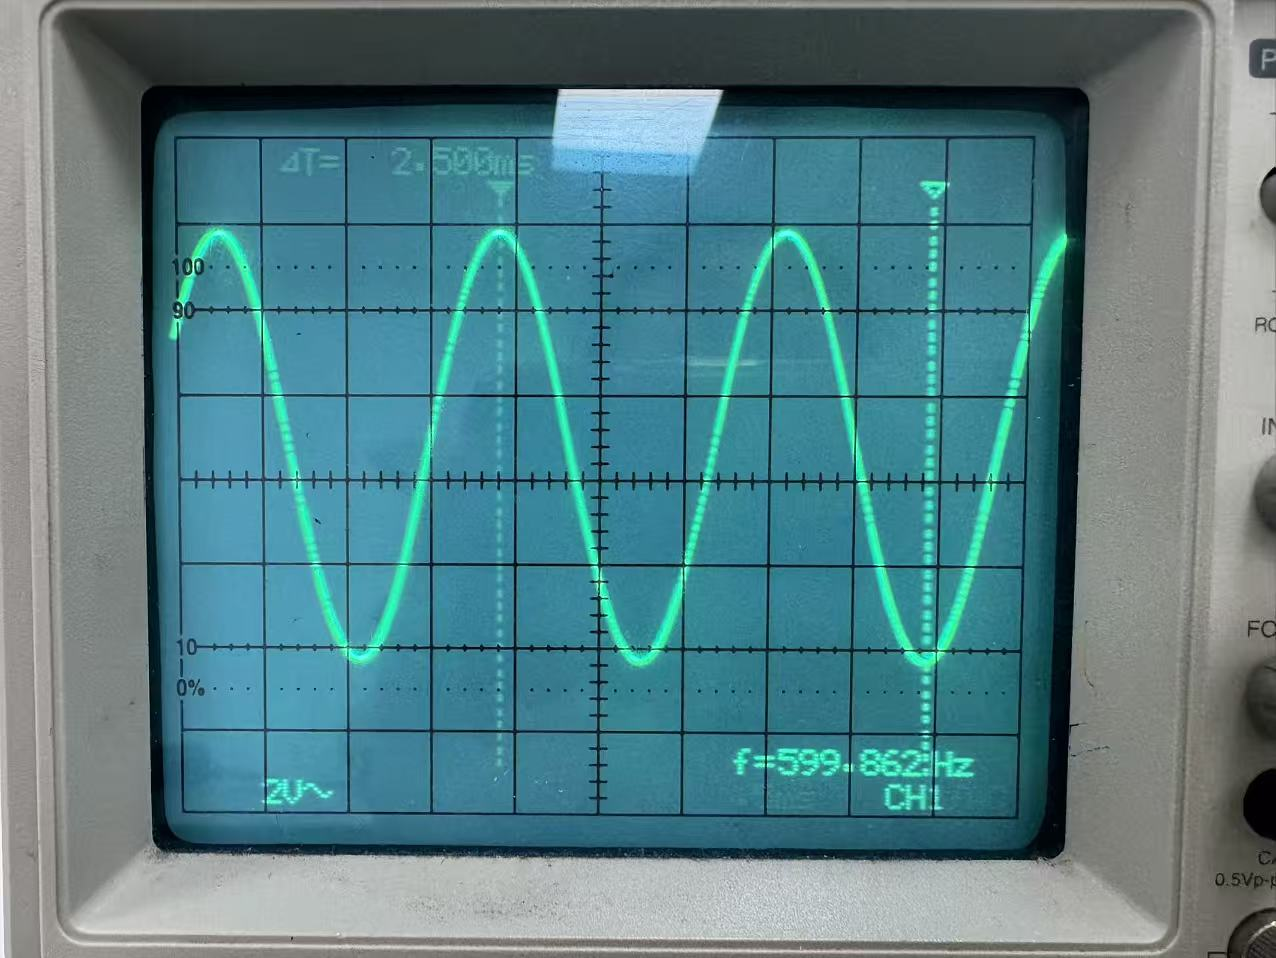
\includegraphics[width=\textwidth]{figures/1-3.jpg} % <-- 替换为您的图片
        \caption{3个完整波形}
        \label{pic:1:3}
    \end{subfigure}

    \vspace{1em} % 在两行子图之间添加一点垂直间距（可选）

    % --- 第二行 ---
    \begin{subfigure}[b]{0.32\textwidth}
        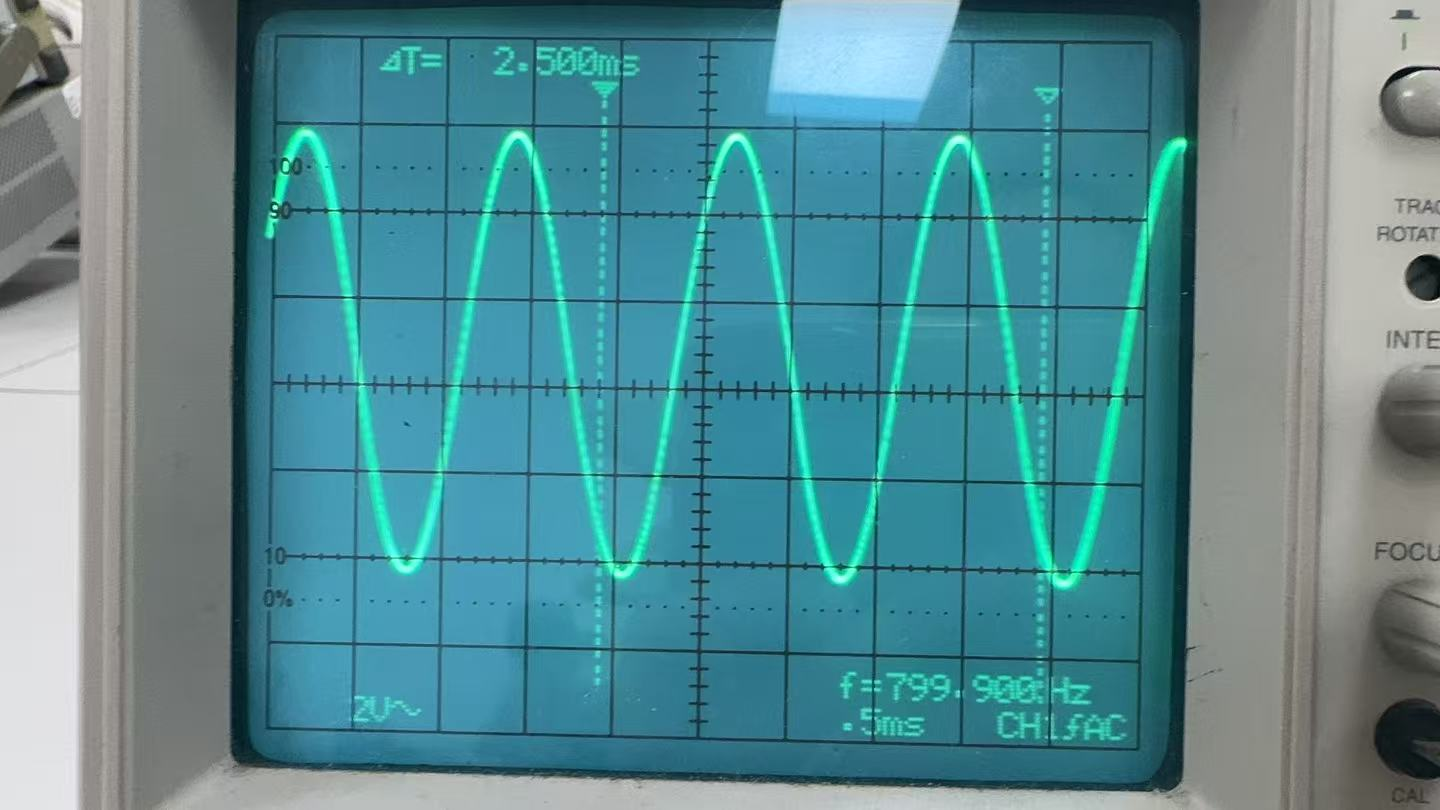
\includegraphics[width=\textwidth]{figures/1-4.jpg} % <-- 替换为您的图片
        \caption{4个完整波形}
        \label{pic:2:1}
    \end{subfigure}
    \hfill % 在子图之间添加水平间距
    \begin{subfigure}[b]{0.32\textwidth}
        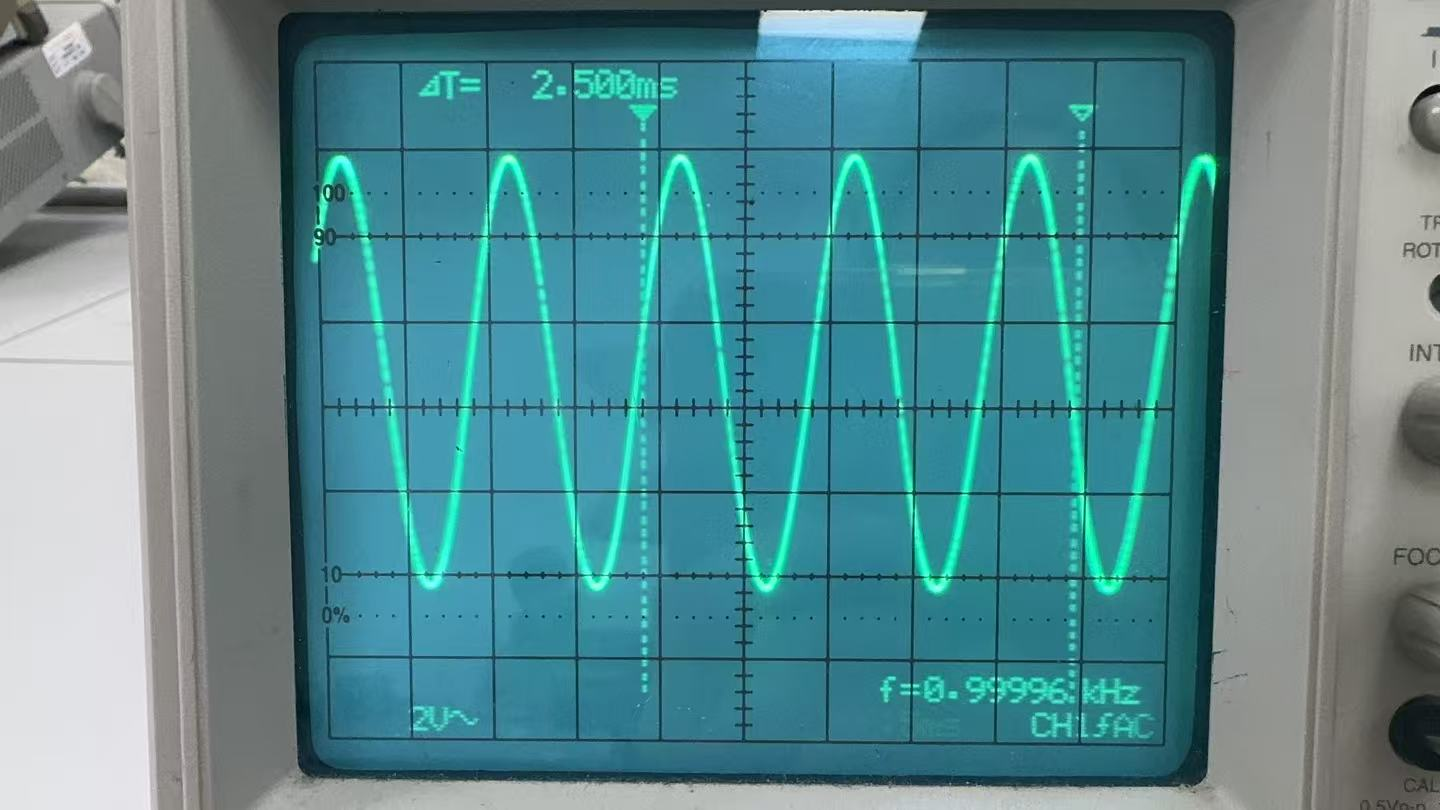
\includegraphics[width=\textwidth]{figures/1-5.jpg} % <-- 替换为您的图片
        \caption{5个完整波形}
        \label{pic:2:3}
    \end{subfigure}
    \hfill % 在子图之间添加水平间距
    \begin{subfigure}[b]{0.32\textwidth}
        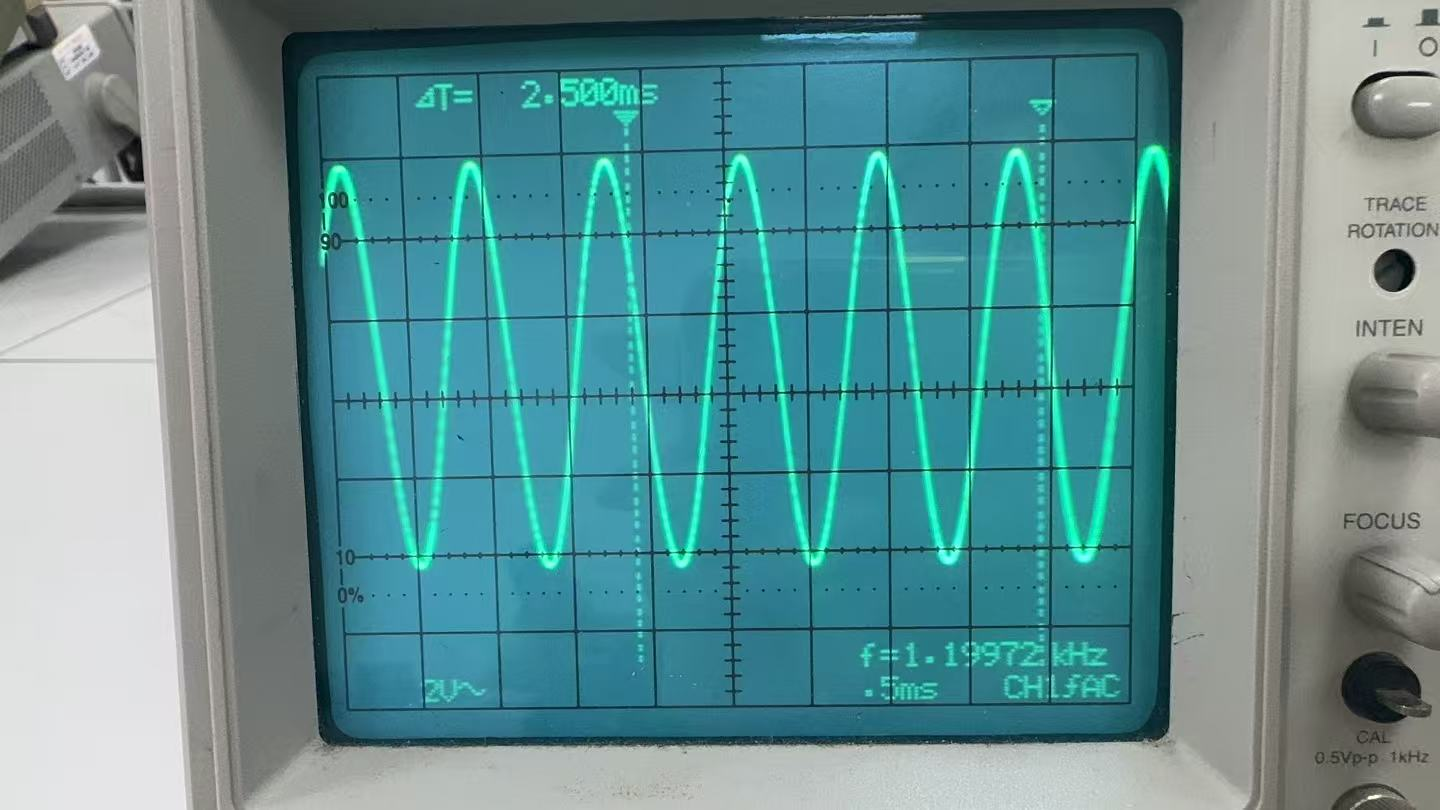
\includegraphics[width=\textwidth]{figures/1-6.jpg} % <-- 替换为您的图片
        \caption{6个完整波形}
        \label{pic:3:2}
    \end{subfigure}

\caption{用李萨如图形测量未知信号的频率} % 整个图的总标题
\end{figure}
测得数据记录在下表：
\begin{table}[H]
\centering
\caption{比较法测量扫描信号频率}
\label{tab:freq}
\begin{tabular}{|l|l|l|}
\hline
波形个数$n$ & 信号频率$f_y$(\si{\hertz}) & 测得的扫描信号频率$f_x$(\si{\hertz}) \\ \hline
1       & 200.700                & 200.700       \\ \hline
2       & 403.100                & 201.550        \\ \hline
3       & 605.300                & 201.767        \\ \hline
4       & 801.400               & 200.350        \\ \hline
5       & 1002.100                &200.420        \\ \hline
6       & 1199.800               & 199.967        \\ \hline
\end{tabular}
\end{table}
\paragraph{平均值}
\begin{equation*}
    \bar{f} = \frac{f_1 + f_2 + \cdots + f_5 + f_6}{6} = 200.792 \text{ Hz}
\end{equation*}

扫描时基信号为 $0.5 \text{ ms/div}$，即理论频率 $f_{\text{理}} = 200 \text{ Hz}$。

\paragraph{相对误差}
\begin{equation*}
    E = \frac{|f_{\text{实}} - f_{\text{理}}|}{f_{\text{理}}} = \frac{|200.792 - 200|}{200} \approx 0.40\%
\end{equation*}

\paragraph{计算 A 类不确定度}
\begin{equation*}
    u_A = \sqrt{\frac{\sum_{i=1}^{6} (\bar{f} - f_i)^2}{6 \times 5}} \approx 0.291 \text{ Hz}
\end{equation*}

\paragraph{最终结果}
\begin{equation*}
    f = (200.79 \pm 0.29) \text{ Hz}
\end{equation*}
\subsubsection{用李萨如图形测量未知信号的频率}
信号发生器背后输出的~50Hz的电压，作为$f_y$
示波器波形如下：

\begin{figure}[H]
    \centering

    % --- 第一行 ---
    \begin{subfigure}[b]{0.32\textwidth}
        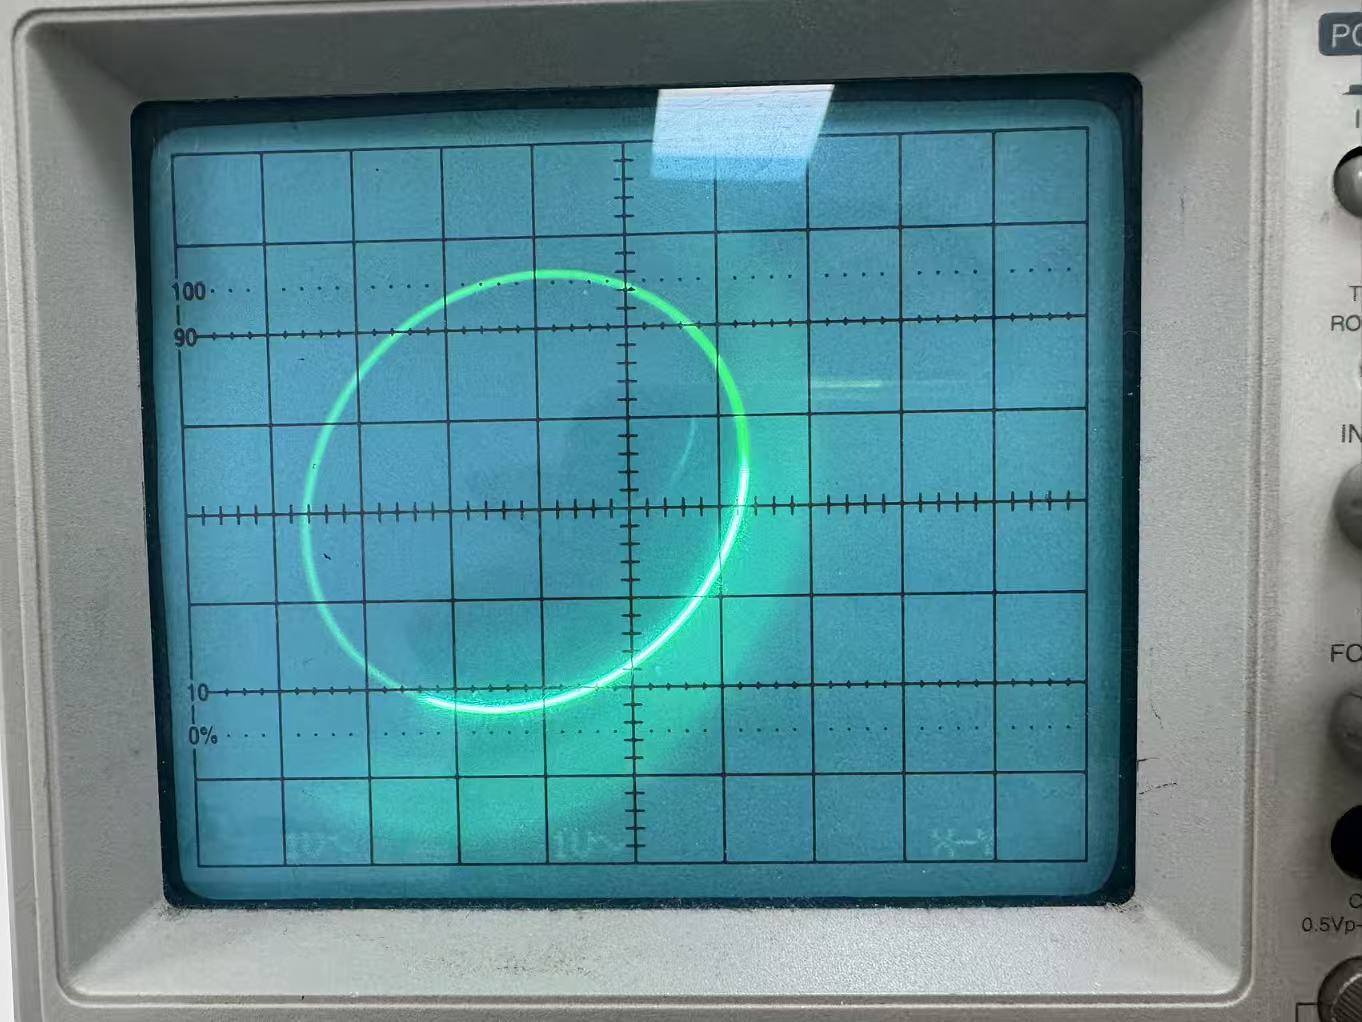
\includegraphics[width=\textwidth]{figures/2-1.jpg}
        \caption{1:1}
        \label{pic:1:1}
    \end{subfigure}
    \hfill % 在子图之间添加水平间距
    \begin{subfigure}[b]{0.32\textwidth}
        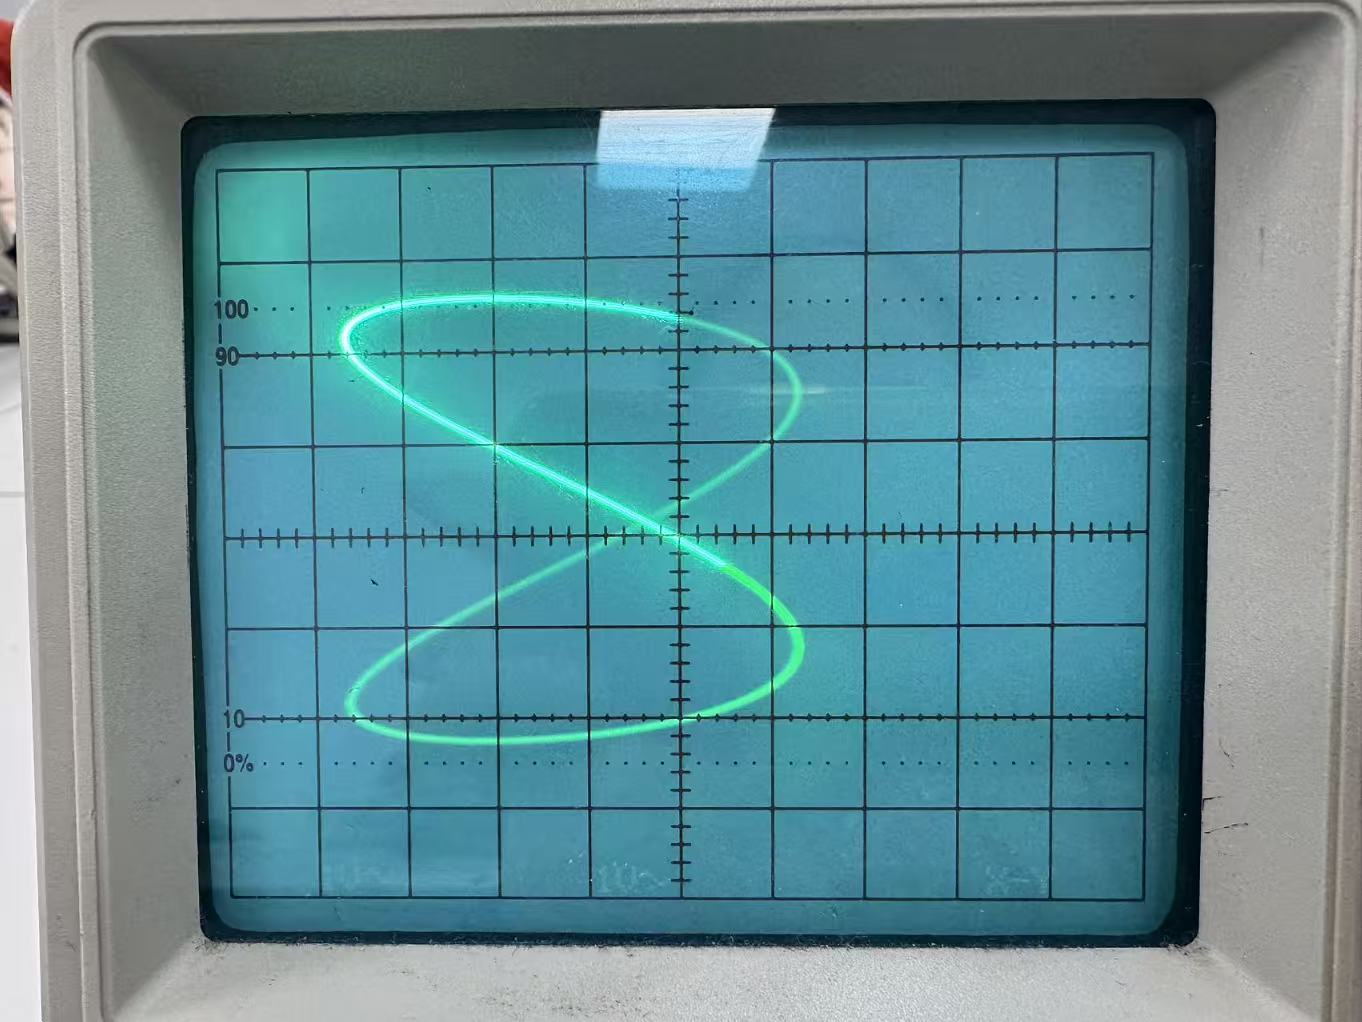
\includegraphics[width=\textwidth]{figures/2-2.jpg}
        \caption{1:2}
        \label{pic:1:2}
    \end{subfigure}
    \hfill % 在子图之间添加水平间距
    \begin{subfigure}[b]{0.32\textwidth}
        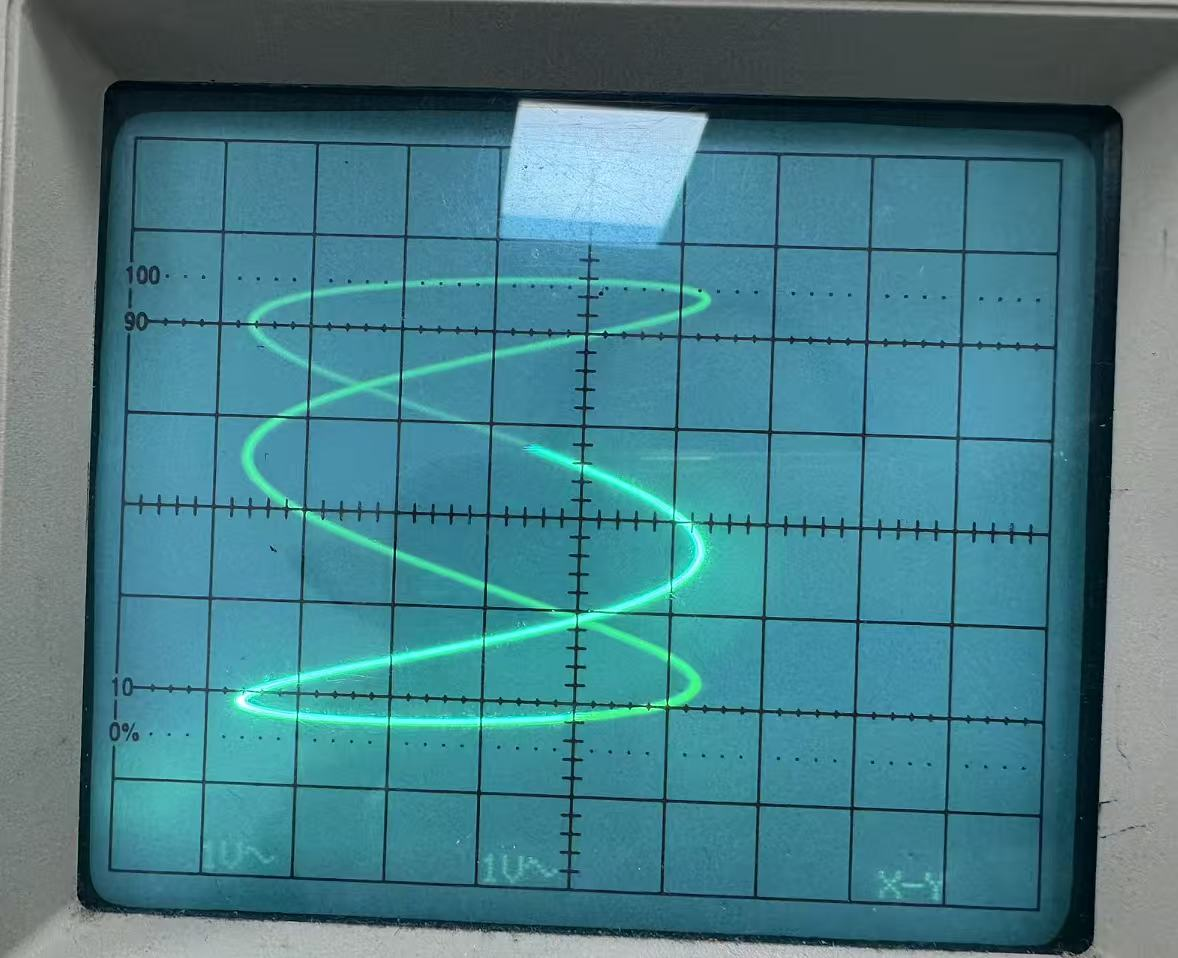
\includegraphics[width=\textwidth]{figures/2-3.jpg} % <-- 替换为您的图片
        \caption{1:3}
        \label{pic:1:3}
    \end{subfigure}

    \vspace{1em} % 在两行子图之间添加一点垂直间距（可选）

    % --- 第二行 ---
    \begin{subfigure}[b]{0.32\textwidth}
        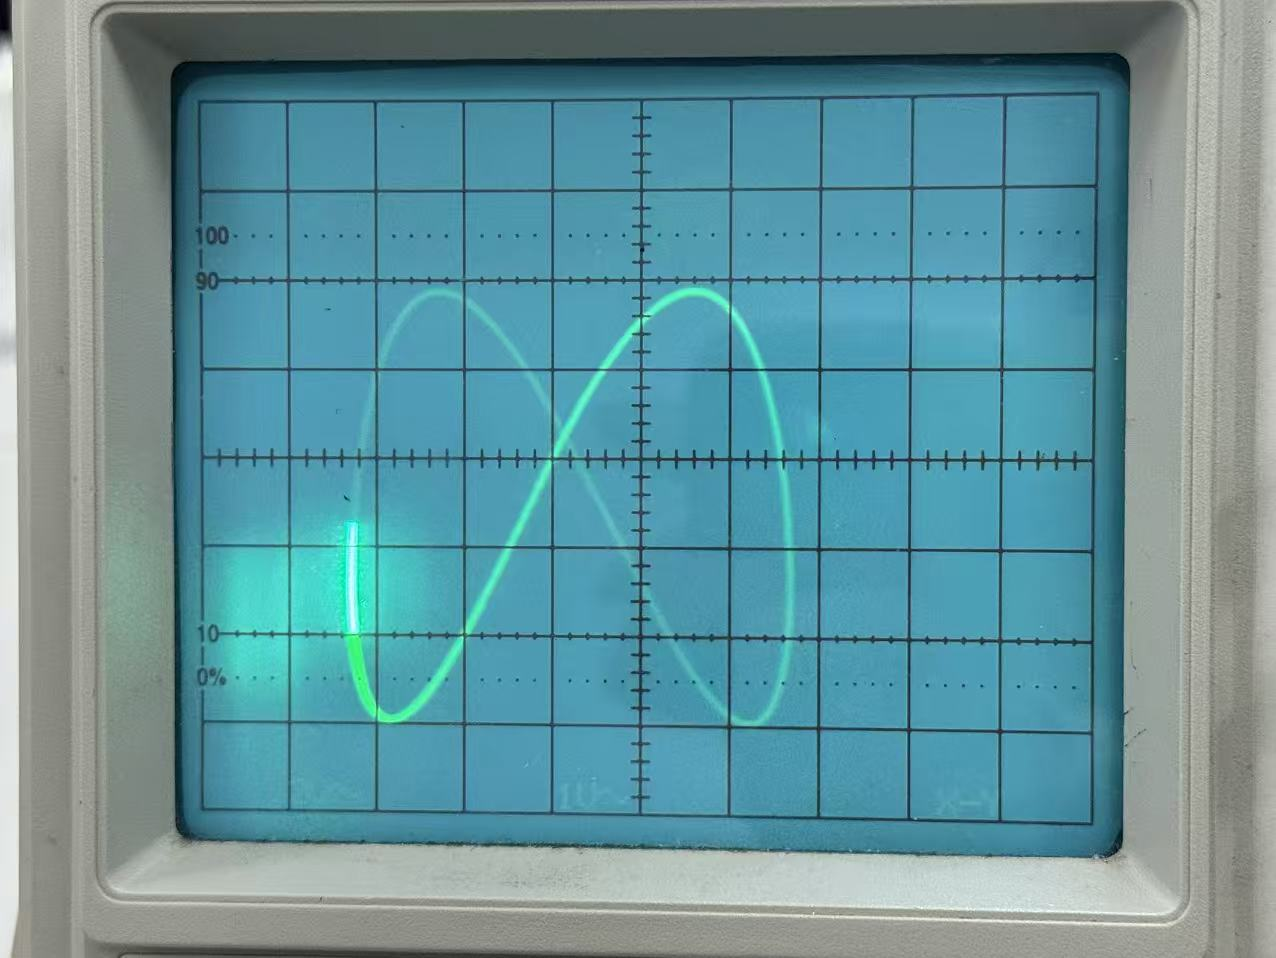
\includegraphics[width=\textwidth]{figures/2-4.jpg} % <-- 替换为您的图片
        \caption{2:1}
        \label{pic:2:1}
    \end{subfigure}
    \hfill % 在子图之间添加水平间距
    \begin{subfigure}[b]{0.32\textwidth}
        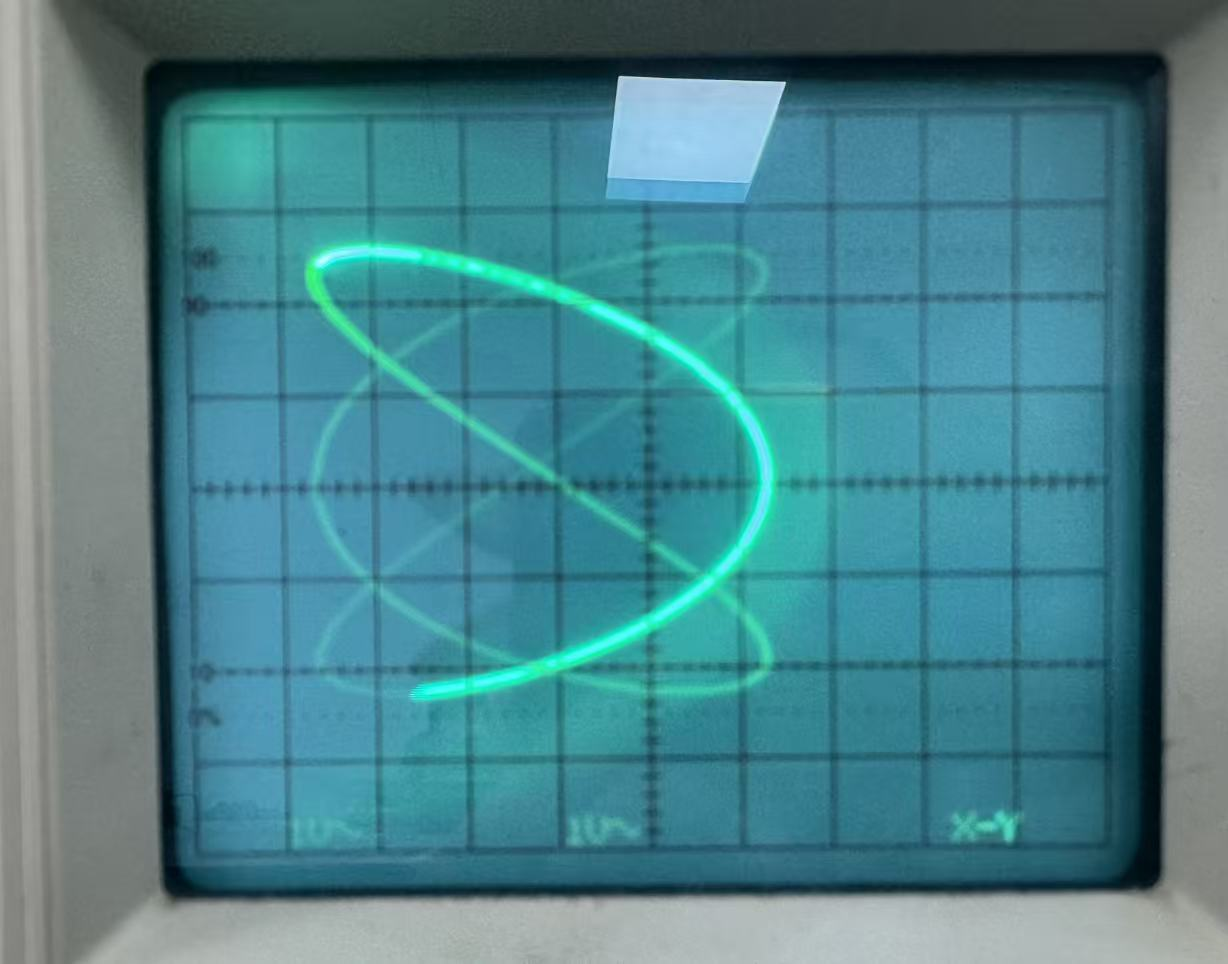
\includegraphics[width=\textwidth]{figures/2-5.jpg} % <-- 替换为您的图片
        \caption{2:3}
        \label{pic:2:3}
    \end{subfigure}
    \hfill % 在子图之间添加水平间距
    \begin{subfigure}[b]{0.32\textwidth}
        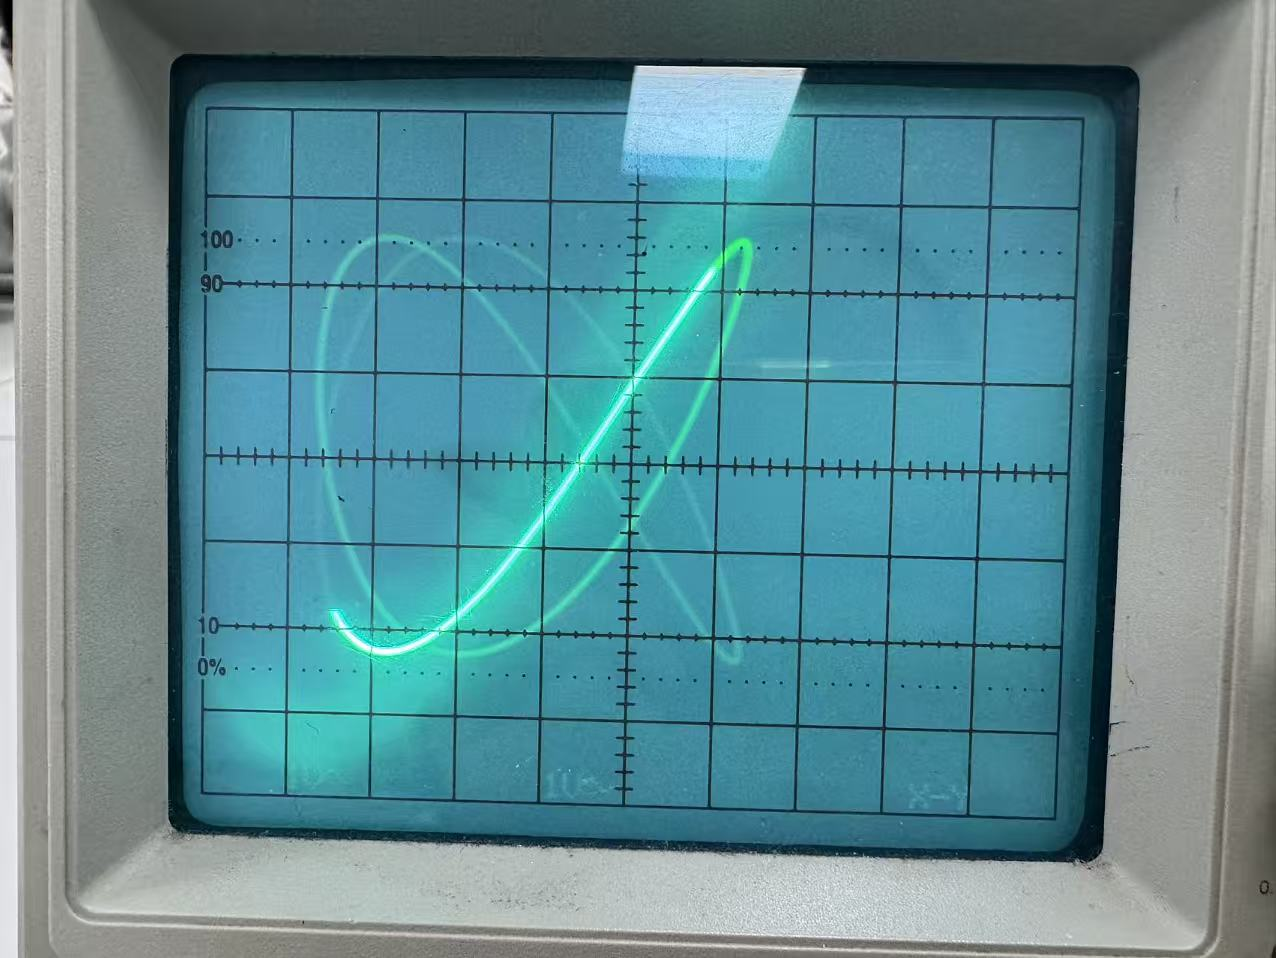
\includegraphics[width=\textwidth]{figures/2-6.jpg} % <-- 替换为您的图片
        \caption{3:2}
        \label{pic:3:2}
    \end{subfigure}

\caption{用李萨如图形测量未知信号的频率} % 整个图的总标题
\end{figure}
测量结果记录在下表：
\begin{table}[H]
\centering
\caption{李萨如图形测量未知信号频率}
\label{tab:li_freq}
\begin{tabular}{|L{0.2\textwidth}|L{0.08\textwidth}|L{0.08\textwidth}|L{0.08\textwidth}|L{0.08\textwidth}|L{0.08\textwidth}|L{0.08\textwidth}|}
\hline
频率比$f_y:f_x$ & 1:3     & 1:2     & 2:3    & 1:1    & 3:2    & 2:1    \\ \hline
图形           & 见\cref{pic:1:3}       & 见\cref{pic:1:2}       & 见\cref{pic:2:3}      & 见\cref{pic:1:1}      & 见\cref{pic:3:2}      & 见\cref{pic:2:1}      \\ \hline
垂直交点数$N_y$   & 6       & 4       & 6      & 2      & 4      & 4      \\ \hline
水平交点数$N_x$   & 2       & 2       & 4      & 2      & 6      & 2      \\ \hline
读出$f_x$(\si{\hertz})      & 150.080 & 99.990 & 75.017 & 50.020 & 33.354 & 25.023 \\ \hline
计算$f_y$(\si{\hertz})      & 50.026  & 49.995  & 50.011 & 50.031 & 50.031 & 50.046 \\ \hline
\end{tabular}
\end{table}
\paragraph{平均值}
\begin{equation*}
    \bar{f}_y = \frac{\sum_{i=1}^{6} f_{yi}}{6} = 50.023 \text{ Hz}
\end{equation*}

\paragraph{相对误差}
\begin{equation*}
    E = \frac{|f_{\text{实}} - f_{\text{理}}|}{f_{\text{理}}} = \frac{|50.023 - 50.000|}{50.000} = 0.046\%
\end{equation*}

\paragraph{计算 A 类不确定度}
\begin{equation*}
    u_A = \sqrt{\frac{\sum_{i=1}^{6} (\bar{f} - f_i)^2}{6 \times 5}} = 0.007 \text{ Hz}
\end{equation*}


\paragraph{最终结果}
\begin{equation*}
    f_y = (50.023 \pm 0.007) \text{ Hz}
\end{equation*}

\subsubsection{测量二极管正向导通电压}
光标法测量结果如下
\begin{figure}[H]
    \centering
    \begin{subfigure}[b]{0.4\textwidth}
        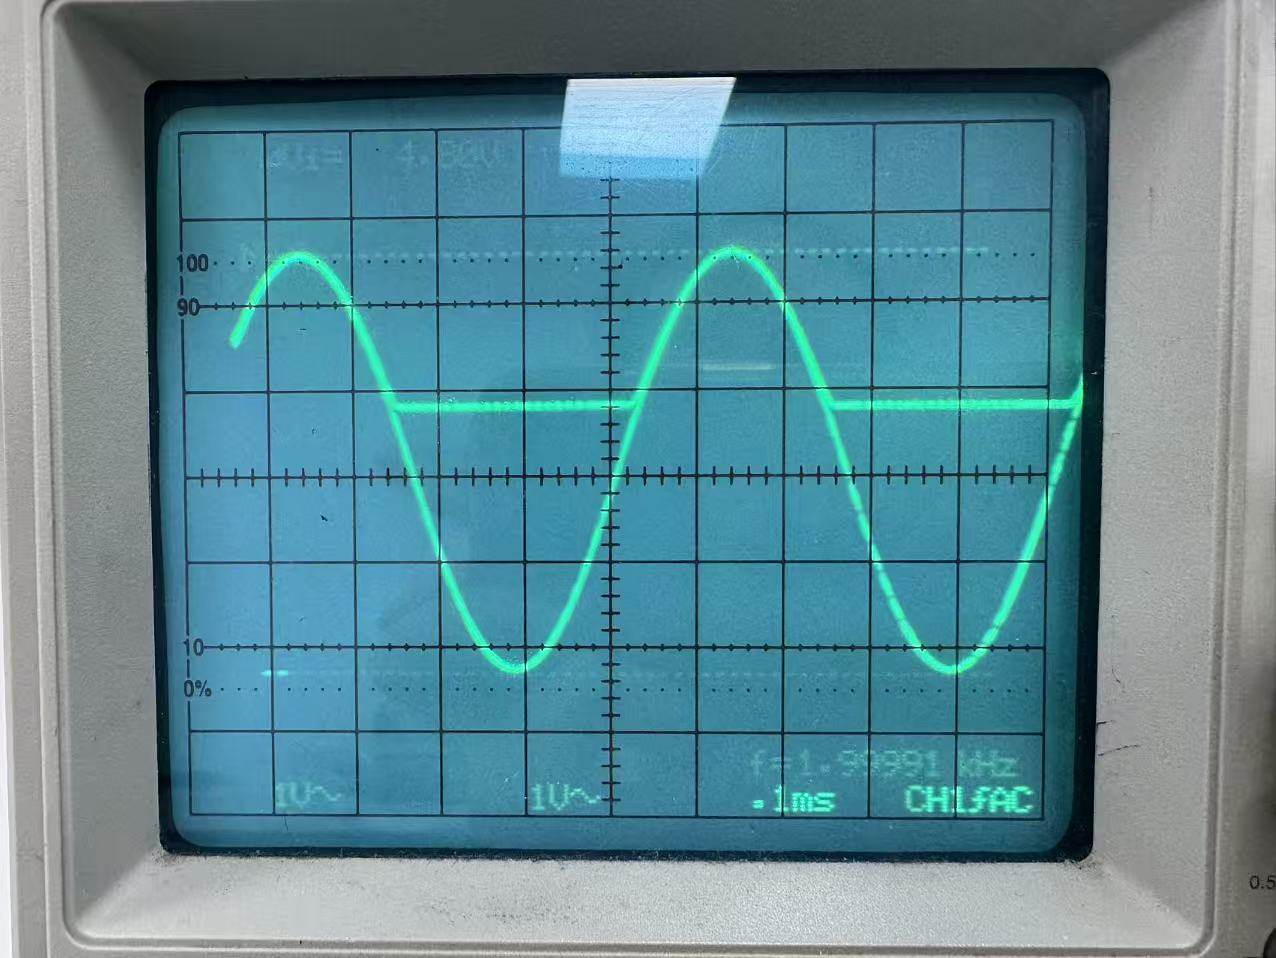
\includegraphics[width=\textwidth]{figures/3-1.jpg}
        \caption{输入电压的峰-峰值}
        \label{pic:pp}
    \end{subfigure}
    \hfill
    \begin{subfigure}[b]{0.4\textwidth}
        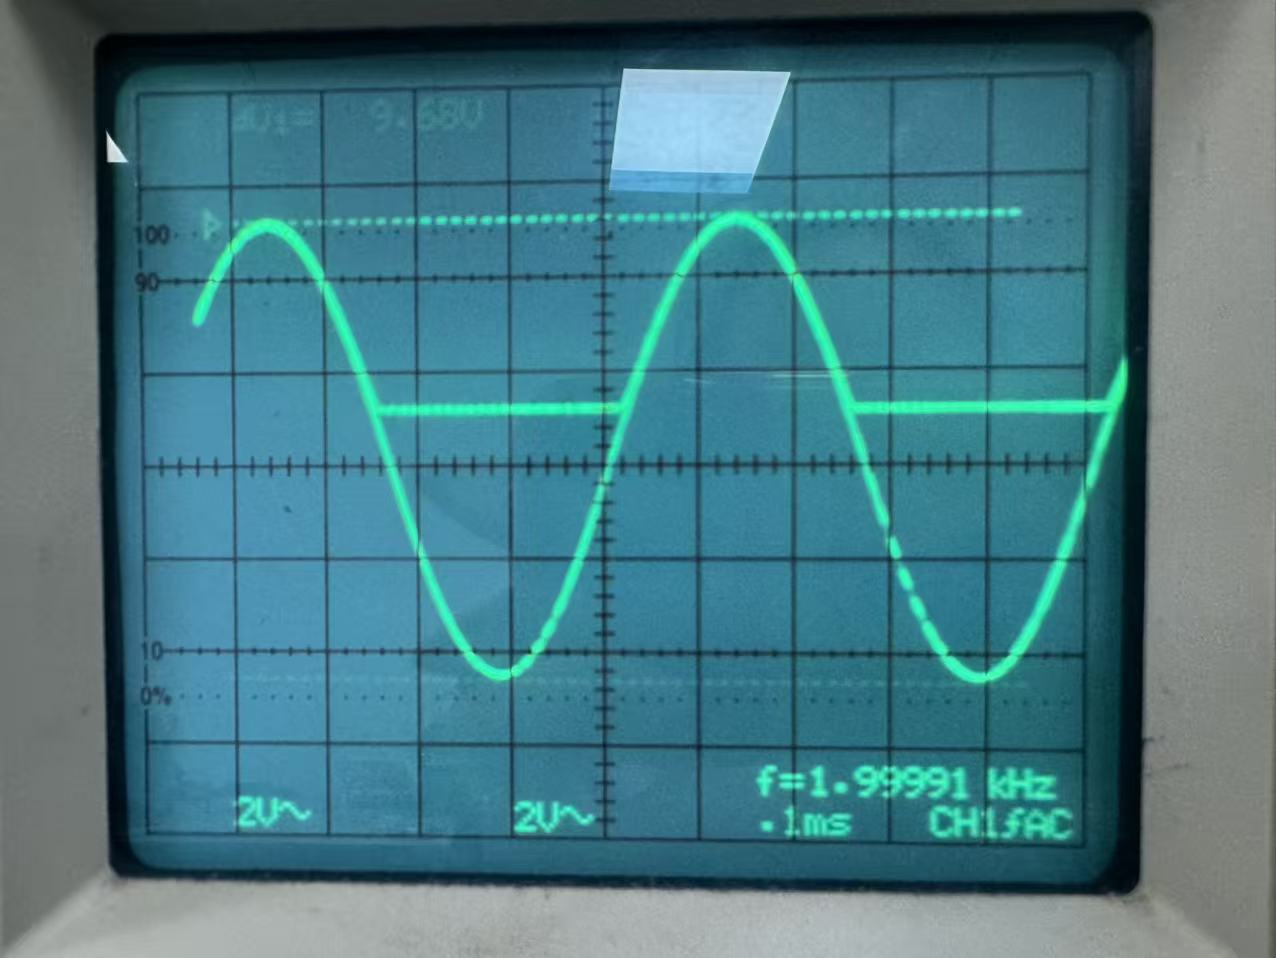
\includegraphics[width=\textwidth]{figures/3-2.jpg}
        \caption{半波电压的峰值}
        \label{pic:p}
    \end{subfigure}
\caption{测量二极管正向导通电压}
\end{figure}
测得数据记录在下表：
$U_\text{导通}=\frac{1}{2}U_{1P-P}-U_{2P}$
\begin{table}[H]
\centering
\caption{二极管导通压降}
\label{tab:di}
\begin{tabular}{|L{0.3\textwidth}|C{.2\textwidth}|C{.2\textwidth}|}
\hline
项目                     & 光标法(\si{\volt }) & 直读法(D=2\si{\volt}) \\ \hline
输入电压的峰-峰值$U_{1P-P}$    & 9.68               &     9.40   \\ \hline
输出半波电压的峰值$U_{2P}$      & 4.00               &     3.84   \\ \hline
二极管导通的电压降$U_\text{导通}$ & 0.84              &    0.86    \\ \hline
\end{tabular}
\end{table}
\subsubsection{测量RC电路相位差}
光标法测量结果如下：
\begin{figure}[H]
    \centering
    \begin{subfigure}[b]{0.4\textwidth}
        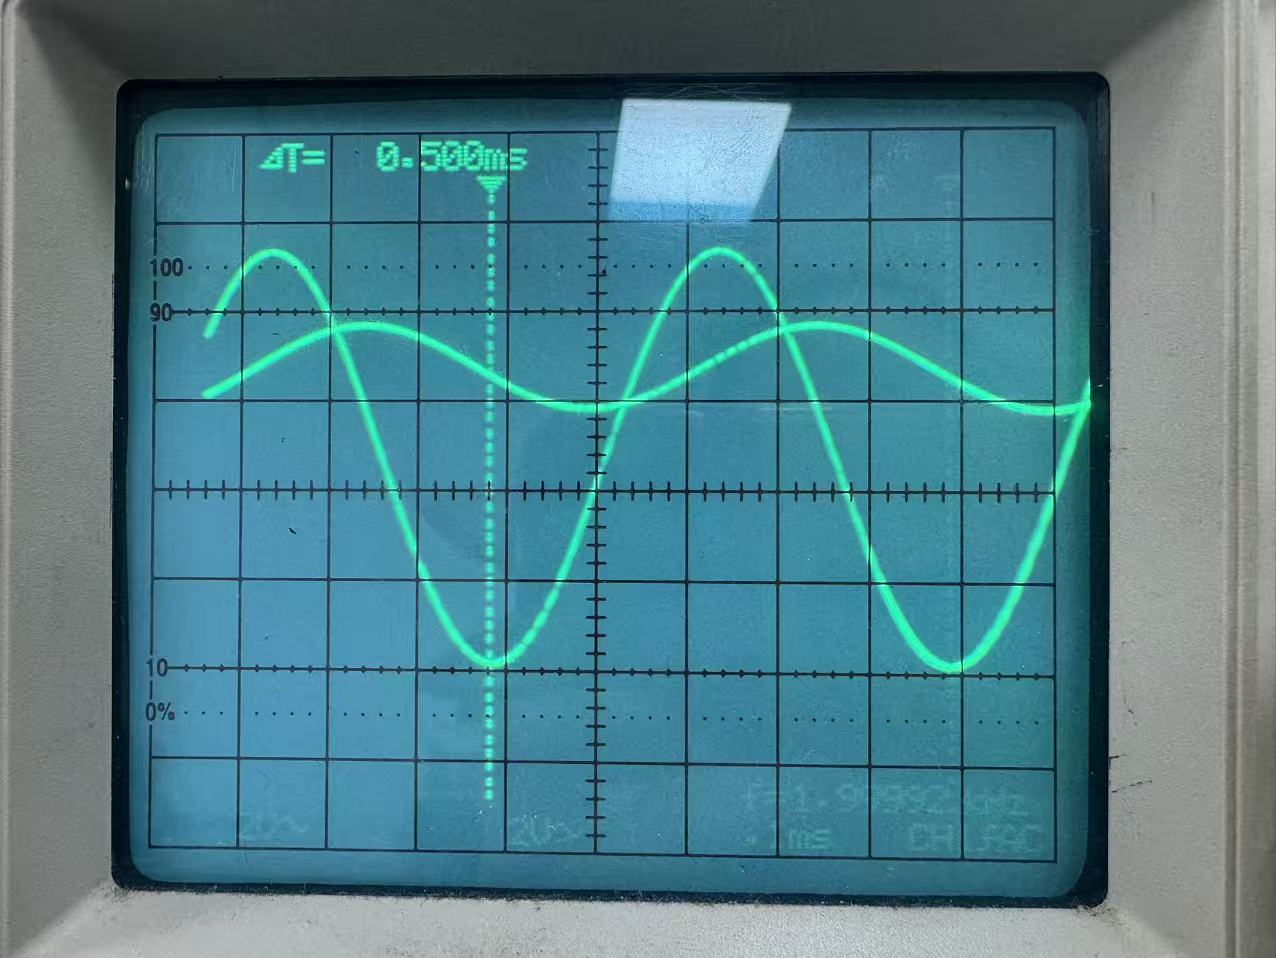
\includegraphics[width=\textwidth]{figures/4-1.jpg}
        \caption{输入信号的周期}
        \label{pic:T}
    \end{subfigure}
    \hfill
    \begin{subfigure}[b]{0.4\textwidth}
        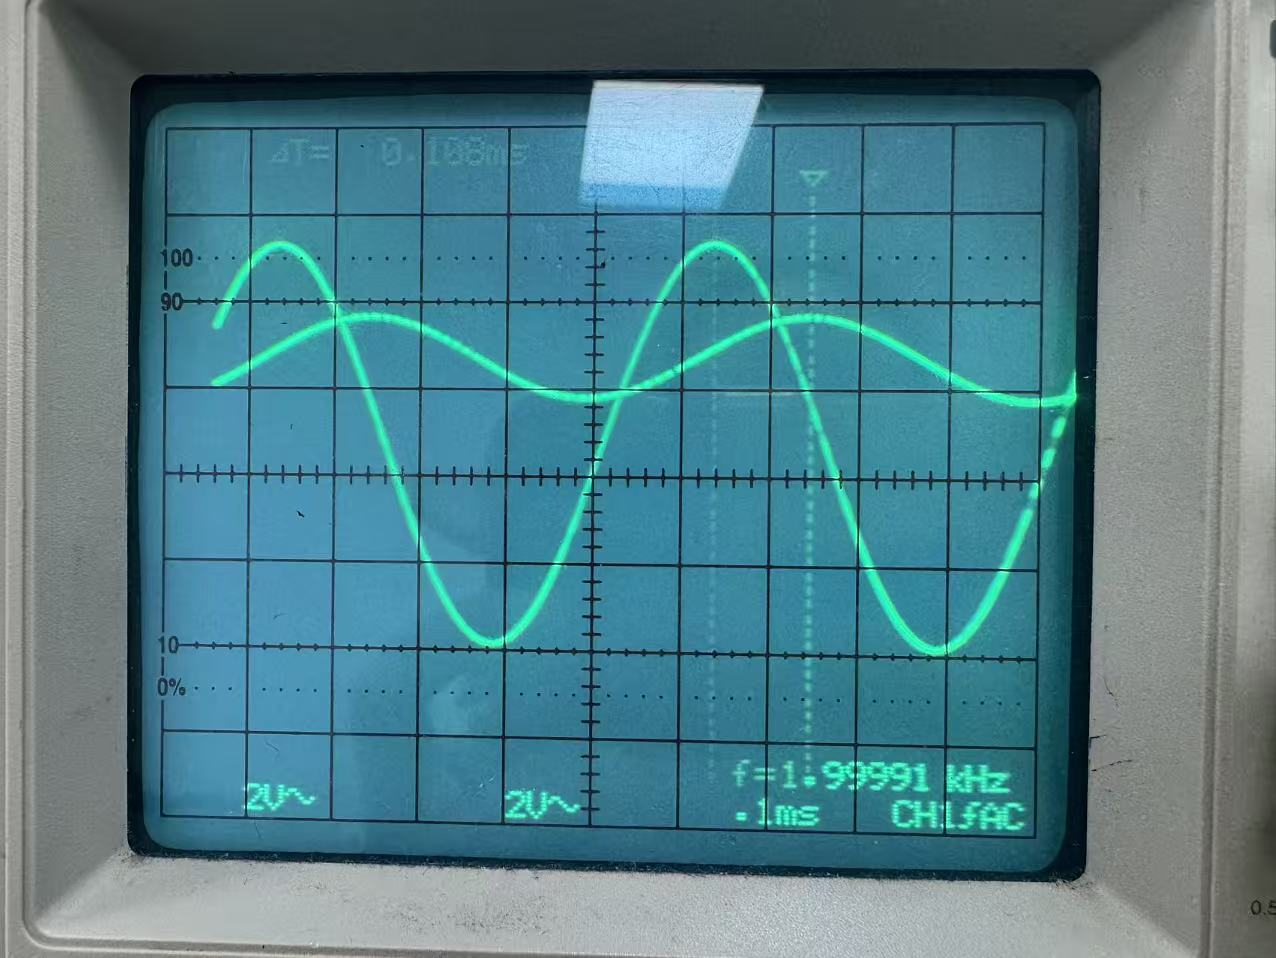
\includegraphics[width=\textwidth]{figures/4-2.jpg}
        \caption{两峰之间的相位差}
        \label{pic:phi}
    \end{subfigure}
\caption{测量RC电路相位差}
\end{figure}
测得数据记录在下表：
$\Delta \phi = \frac{\Delta t}{T} \times 360^\circ$
\begin{table}[H]
\centering
\caption{测量RC电路相位差}
\label{tab:phi}
\begin{tabular}{|l|l|l|}
\hline
                                & 光标法 &直读法(D=0.1ms) \\ \hline
周期$T$(\si{\milli\second})      &  0.500       & 0.510             \\ \hline
$\Delta t$(\si{\milli\second})   &   0.108      &  0.105             \\ \hline
相位差$\Delta \varphi$ ($^\circ$)          & 77.760       & 78.431            \\ \hline
\end{tabular}
\end{table}
\subsection{误差分析（20分）}

在本实验中，测量数据与理论预期展现出了较高的一致性。例如，在李萨如图形法测频率实验中，计算所得的相对误差仅为 \SI{0.046}{\percent}，这表明实验系统的整体准确度较高。然而，深入剖析测量过程，仍可识别出以下几类影响结果精度的误差来源：

\begin{enumerate}
    \item \textbf{系统性仪器误差}
    
    这是本实验误差的最主要来源，其影响贯穿于信号产生与处理的全过程：
    \begin{itemize}
        \item \textbf{信号源输出与示值的不一致性：} 实验中所使用的函数信号发生器并非绝对频率基准。其显示的设定值与内部压控振荡器（VCO）或直接数字频率合成（DDS）产生的实际物理频率之间存在固有的频率偏差。在实验一中，时基频率理论值 $f_x$ 为 \SI{200}{\hertz}，而实测均值 $\bar{f} = \SI{195.746}{\hertz}$，约 \SI{2.1}{\percent} 的偏离值反映了仪器时钟参考源的校准残留误差。
        \item \textbf{频率的热漂移现象：} 受限于电子元件的热稳定性，信号发生器在工作过程中会产生微小的频率漂移。在李萨如图形实验中观察到，原本处于静态或极缓慢旋转的图形，在运行一段时间后翻转速度发生变化，这种动态不稳定性为捕捉瞬时同步状态带来了技术挑战。
    \end{itemize}

    \item \textbf{分辨力限制与随机读数误差}
    
    读数过程中的主观判断与显示终端的物理限制构成了随机误差的主体：
    \begin{itemize}
        \item \textbf{荧光屏轨迹的物理线宽效应：} 示波器呈现的并非理想的几何线，而是具有一定弥散圆直径的电子束轨迹。在利用光标（Cursors）定位波峰或波谷时，光标线与具有一定宽度的波形边缘重合处存在模糊带，这在测量电压峰-峰值 $V_{pp}$ 或相位角时，引入了不可避免的空间分辨率误差。
        \item \textbf{触发抖动与相位对准误差：} 在手动调节触发电平以稳定波形时，由于信号噪声的存在，触发点可能产生极细微的抖动。在测量周期 $T$ 时，波形起始相位与网格刻度线的手动对齐过程依赖实验者的视觉判定，这种空间映射的不确定性直接影响了频率换算的精度。
    \end{itemize}

    \item \textbf{量程校准与非线性响应}
    
    示波器内部的放大电路（垂直系统）和扫描电路（水平系统）存在微小的非线性失真：
    \begin{itemize}
        \item 垂直灵敏度（\si{\volt\per div}）与水平扫描速度（\si{\ms\per div}）在各量程档位间的切换并非绝对线性。虽然本实验所用仪器性能良好，但在大跨度量程切换时，衰减器和放大器的增益误差仍可能对测量结果产生微扰。
    \end{itemize}

    \item \textbf{结论与改进策略}
    
    综上所述，本实验的误差由仪器频率基准偏差与人工读数限制共同构成。为进一步提升实验精度，实验中采取了多次测量求平均值的方法以削弱随机误差的影响；同时，优先选择光标自动测量而非肉眼估读格数，有效地控制了相对误差。最终结果显示，实验数据在工程允许范围内具有极高的可靠性。

\end{enumerate}

\subsection{实验探讨（10分）}

本实验通过调节示波器的时基与触发系统，实现了复杂电信号的稳定捕捉。利用光标测量功能，定量分析了波形的幅值与频率特性；通过李萨如图形探究了频率合成规律。实验不仅掌握了仪器使用，更从现象中验证了电子束偏转与同步显示的物理本质。
\section{思考题（10分）}

\subsection{示波器的主要结构与各部分的作用是什么？示波器为什么能显示被测信号的波形？}

\paragraph{1. 主要结构及其作用：}
示波器（以模拟示波器为例）的核心结构是示波管（CRT），主要由以下三部分组成：
\begin{itemize}
    \item \textbf{电子枪：} 负责发射、加速并聚焦电子流，形成极细的电子束。
    \item \textbf{偏转系统：} 包括垂直（Y轴）和水平（X轴）偏转板。Y轴负责随信号幅值上下偏转电子束，X轴负责随时间线性拉伸电子束。
    \item \textbf{荧光屏：} 电子束撞击荧光物质发光，将电子的运动轨迹转化为可见光图像。
\end{itemize}

\paragraph{2. 显示原理：}
示波器采用“扫描显示”技术。当被测电压 $u_y(t)$ 施加在垂直偏转板上时，电子束的垂直位移 $y$ 正比于电压幅值；同时，水平偏转板施加一个线性增长的锯齿波扫描电压 $u_x(t) = kt$，使电子束在水平方向匀速移动。
这样，屏幕上的点在 X 方向代表时间，在 Y 方向代表电压，电子束扫过的轨迹即复现了函数 $u_y(t)$ 的波形图像。

\subsection{在观察李萨如图形时为什么总是不断地来回翻动，翻动的快慢是受哪种因素所影响？}

\paragraph{翻动原因：} 李萨如图形的形态由两个相互垂直的正弦振动的频率比 $f_y/f_x$ 和相位差 $\Delta\phi$ 决定。由于实验中使用的两个信号源频率很难做到绝对的同步或成完美的整数比，它们之间存在极细微的频率偏差。这导致两信号间的相位差 $\Delta\phi$ 随时间不断漂移，使图形在直线、椭圆、圆之间循环变换，宏观上表现为图形的翻转或滚动。

\paragraph{影响因素：} 翻动的快慢取决于相位差改变的速率。具体而言，它受信号频率偏离理想整数比的程度所影响。设理想频率比为 $p:q$（$p, q$ 为互质整数），则翻动频率与 $\Delta f = |p f_x - q f_y|$ 成正比。频率差越大，相位漂移越快，图形翻转就越剧烈。

\subsection{切实理解示波器同步的概念，如果发生波形左移或右移时应如何调整才能使其稳定下来？}

\paragraph{同步概念：} “同步”的物理本质是要求示波器扫描周期的起始点与被测信号的某一相位点保持固定的时间对应关系。如果扫描周期 $T_x$ 与信号周期 $T_y$ 满足 $T_x = n T_y$（$n$ 为整数），且每次扫描都从相同的相位点开始，屏幕上留下的多段波形轨迹就会完全重合，形成稳定的视觉图像。

\paragraph{调整方法：} 若观察到波形在水平方向滚动（左移或右移），说明扫描频率与信号频率不匹配，或者触发点不稳定。应按以下步骤调整：
\begin{enumerate}
    \item \textbf{调节触发电平（TRIG LEVEL）：} 改变触发阈值，使触发线处于被测信号的峰-峰值之间，确保电路能够捕获到触发特征点。
    \item \textbf{选择触发源（Source）：} 确保触发源选定为当前显示信号所在的通道（如 CH1）。
    \item \textbf{调节触发斜率（Slope）：} 选择上升沿或下降沿触发，以适应特定的信号特征。
    \item \textbf{微调时基（Time/Div）：} 若偏差过大，可适当调节水平扫描速度，使波形周期数处于易于观察的范围。
\end{enumerate}

\begin{figure}[H]
    \centering
    \begin{tikzpicture}[scale=1.2]
        % 绘制网格
        \draw[very thin, lightgray!40] (0,-1.5) grid (6,1.5);
        
        % 画坐标轴
        \draw[->,thick] (0,0) -- (6,0) node[right] {$t$};
        \draw[->,thick] (0,-1.5) -- (0,1.5) node[above] {$U$};
        
        % 画正弦波 (模拟输入信号)
        \draw[blue, thick, domain=0:5.5, samples=100] plot (\x, {sin(\x r * 3)});
        
        % 画触发电平线
        \draw[red, dashed, thick] (0, 0.6) -- (5.5, 0.6) node[right, font=\small] {Level};
        
        % 标注触发点 (交点)
        \fill[red] (0.22, 0.6) circle (2pt);
        \fill[red] (2.31, 0.6) circle (2pt);
        \fill[red] (4.41, 0.6) circle (2pt);
        
        % 扫描起始标注
        \draw[<-] (0.22, 0.7) -- (1, 1.3) node[right, font=\footnotesize] {每次扫描均由此相位起始};
        
        % 周期标注
        \draw[<->, gray, thick] (0.22, -1.1) -- (2.31, -1.1) node[midway, below, font=\footnotesize] {信号周期 $T$};
        
        % 示意触发脉冲
        \foreach \x in {0.22, 2.31, 4.41}
            \draw[green!50!black, thick] (\x, -1.8) -- (\x, -1.4) -- (\x+0.1, -1.4) -- (\x+0.1, -1.8);
        \node at (5.3, -1.6) [font=\footnotesize] {触发脉冲};
    \end{tikzpicture}
    \caption{示波器触发同步机制及电平调节示意图}
\end{figure}






\insertnotes
\end{document}